\begin{frame}
    \frametitle{Kempe-chains}

    \begin{definition}
        Let $G_{ab}(x)$ be the subgraph consisting of all the vertices colored $ab$ in the coloring $x$ of $G$.
        Then the \emph{Kempe-chain} $\kappa_{ab}(v)$ or \emph{$ab$-chain} of the vertex $v$ is the component of $G_{ab}(x)$ that contains $v$. 
    \end{definition}
    
    \begin{figure}[!ht]
        \centering
        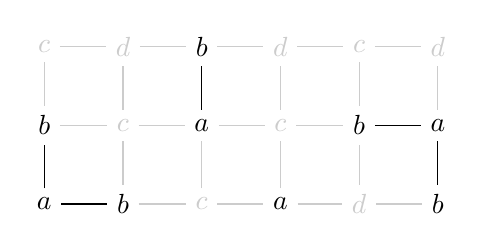
\begin{tikzpicture}[scale=1]
            \node (x11) at (0, 0) { $a$ };
            \node (x12) at (1, 0) { $b$ };
            \node[opacity=0.2] (x13) at (2, 0) { $c$ };
            \node (x21) at (0, 1) { $b$ };
            \node[opacity=0.2] (x22) at (1, 1) { $c$ };
            \node (x23) at (2, 1) { $a$ };
            \node[opacity=0.2] (x31) at (0, 2) { $c$ };
            \node[opacity=0.2] (x32) at (1, 2) { $d$ };
            \node (x33) at (2, 2) { $b$ };
            \node (y11) at (3, 0) { $a$ };
            \node[opacity=0.2] (y12) at (4, 0) { $d$ };
            \node (y13) at (5, 0) { $b$ };
            \node[opacity=0.2] (y21) at (3, 1) { $c$ };
            \node (y22) at (4, 1) { $b$ };
            \node (y23) at (5, 1) { $a$ };
            \node[opacity=0.2] (y31) at (3, 2) { $d$ };
            \node[opacity=0.2] (y32) at (4, 2) { $c$ };
            \node[opacity=0.2] (y33) at (5, 2) { $d$ };
    
            \draw (x11) -- (x12);
            \draw[opacity=0.2] (x12) -- (x13);
    
            \draw[opacity=0.2] (x21) -- (x22);
            \draw[opacity=0.2] (x22) -- (x23);
            \draw[opacity=0.2] (x31) -- (x32);
            \draw[opacity=0.2] (x32) -- (x33);
    
            \draw (x11) -- (x21);
            \draw[opacity=0.2] (x21) -- (x31);
            \draw[opacity=0.2] (x12) -- (x22) -- (x32);
            \draw[opacity=0.2] (x13) -- (x23);
            \draw (x23) -- (x33);
    
            \draw[opacity=0.2] (y11) -- (y12) -- (y13);
            \draw[opacity=0.2] (y21) -- (y22);
            \draw (y22) -- (y23);
            \draw[opacity=0.2] (y31) -- (y32) -- (y33);
    
            \draw[opacity=0.2] (y11) -- (y21) -- (y31);
            \draw[opacity=0.2] (y12) -- (y22) -- (y32);
            \draw (y13) -- (y23);
            \draw[opacity=0.2] (y23) -- (y33);
    
            \draw[opacity=0.2] (x13) -- (y11);
            \draw[opacity=0.2] (x23) -- (y21);
            \draw[opacity=0.2] (x33) -- (y31);
        \end{tikzpicture}
        \caption{We write $\chain{v_1}{v_2}{ab}$ to indicate $v_1$ and $v_2$ lie on the same $ab$-chain.}
    \end{figure}
    
\end{frame}

\begin{frame}
    \frametitle{Ring schemes}

    \begin{definition}
        Given a coloring $x$ of a planar graph $G$ and the colors on its ring $x(R)$. The \emph{scheme} on $R$ of $x$ consists of $x(R)$ with knowledge whether $u \in \kappa_{ab}(v)$ for two ring vertices $u,v \in R$ and colors $ab$.
    \end{definition}
    \begin{figure}[!ht]
        \centering
        \begin{tikzpicture}[scale=1.0, mid arrow/.style={
            postaction={ decorate, decoration={ markings, mark=at position 0.6 with { \arrow[black]{>>} } } } }]
    
            \node[circle, fill, scale=0.015cm, opacity=0.2] (v) at (0, 0) { };
            \node[circle, fill, scale=0.015cm, label=above:$a$] (l1) at (0, 1) { };
            \node[circle, fill, scale=0.015cm, label=right:$b$] (l2) at (0.9, 0.30) { };
            \node[circle, fill, scale=0.015cm, label=below:$c$] (l3) at (0.6, -0.77) {};
            \node[circle, fill, scale=0.015cm, label=below:$a$] (l4) at (-0.6, -0.77) {};
            \node[circle, fill, scale=0.015cm, label=left:$b$] (l5) at (-0.9, 0.30) {};
            \node[circle, fill, scale=0.015cm, label=above:$c$] (c1) at (0.7, 1) {};
            \node[circle, fill, scale=0.015cm, label=right:$a$] (c2) at (1.32, 0.68) {};
            \node[circle, fill, scale=0.015cm, label=right:$c$] (c3) at (1.45, 0.05) {};
            \node[circle, fill, scale=0.015cm, label=right:$a$] (c4) at (1.1, -0.49) {};
            \draw[mid arrow] (l1) -- (l2);
            \draw (l2) -- (l3) -- (l4) -- (l5) -- (l1);
            \draw (l1) -- (c1) -- (c2) -- (c3) -- (c4) -- (l3);
            \draw[opacity=0.2] (l1) -- (v);
            \draw[opacity=0.2] (l2) -- (v);
            \draw[opacity=0.2] (l3) -- (v);
            \draw[opacity=0.2] (l4) -- (v); 
            \draw[opacity=0.2] (l5) -- (v);
            \node (impl) at (3, 0) { $\hspace{1cm} \implies \hspace{0.3cm} \begin{matrix}
                \scheme{a,b,c,a,b}{ 13a } \\
                \scheme{a,b,c,a,b}{ 25d- }
            \end{matrix}$ };
        \end{tikzpicture}
    \caption{The edge with $\gg$ indicates order of vertices in the coloring.}
    \end{figure}
\end{frame}

\begin{frame}
    \frametitle{Schemes imply new colorings}
    \begin{definition}
        Given two schemes $x$ and $y$. We say that $x$ implies $y$ if $x=y$ or $y$ can be obtained from $x$ by flipping a Kempe-chain. Write $x\compat y$.
    \end{definition}
    
    \begin{equation*}
        \scheme{a,b,c,a,b}{ 13a } \compat \scheme{a,b,c,a,\textbf{d}}{{13a}}, \quad \quad
        \scheme{a,b,c,a,b}{ 25d- } \compat \scheme{a,\textbf{d},c,a,b}{{25d-}}.
    \end{equation*}

    \vspace{1cm}
    This is the key argument we used in the five color theorem!
\end{frame}